\documentclass[12pt,a4paper]{article}

\usepackage[utf8]{inputenc}
\usepackage[spanish]{babel}
\usepackage{graphicx}
\usepackage{geometry}
\geometry{a4paper, margin=2.5cm}
\usepackage{xcolor}
\usepackage{listings}
\usepackage{booktabs}
\usepackage{amsmath}
\usepackage{subcaption}
\usepackage{float}
\usepackage[colorlinks=true, linkcolor=blue, urlcolor=blue]{hyperref}

\definecolor{codegreen}{rgb}{0,0.6,0}
\definecolor{codegray}{rgb}{0.5,0.5,0.5}
\definecolor{codepurple}{rgb}{0.58,0,0.82}
\definecolor{backcolour}{rgb}{0.95,0.95,0.92}

\lstdefinestyle{mystyle}{
    backgroundcolor=\color{backcolour},   
    commentstyle=\color{codegreen},
    keywordstyle=\color{magenta},
    numberstyle=\tiny\color{codegray},
    stringstyle=\color{codepurple},
    basicstyle=\ttfamily\footnotesize,
    breakatwhitespace=false,         
    breaklines=true,                 
    captionpos=b,                    
    keepspaces=true,                 
    numbers=left,                    
    numbersep=5pt,                  
    showspaces=false,                
    showstringspaces=false,
    showtabs=false,                  
    tabsize=2,
    literate={á}{{\'a}}1 {é}{{\'e}}1 {í}{{\'i}}1 {ó}{{\'o}}1 {ú}{{\'u}}1
             {Á}{{\'A}}1 {É}{{\'E}}1 {Í}{{\'I}}1 {Ó}{{\'O}}1 {Ú}{{\'U}}1
             {ñ}{{\~n}}1 {Ñ}{{\~N}}1
}
\lstset{style=mystyle}

\title{\Huge\textbf{PROYECTO ESP32} \\ \Large Temperatura con Termómetro Gráfico \\ \vspace{0.5cm} \normalsize \textit{Termo-higrómetro con termómetro gráfico animado en pantalla OLED SSD1306}}
\author{Msc. Néstor Fabio Montoya Palacios}
\date{2026 \\ \vspace{0.2cm} \small Plataforma: ESP32 Dev Module}

\begin{document}

\maketitle
\tableofcontents
\newpage

% ══════════════════════════════════════════════════════════════
\section{Introducción}
% ══════════════════════════════════════════════════════════════

Este documento describe de manera detallada el proyecto ``Temperatura con Termómetro'', una evolución del proyecto básico de lectura de temperatura que incorpora un \textbf{termómetro gráfico animado} en la pantalla OLED. El sistema utiliza un sensor digital DHT22 (AM2302) conectado a un microcontrolador ESP32, con los resultados mostrados en una pantalla OLED de 0.96 pulgadas mediante una representación visual que incluye un termómetro clásico con nivel de ``mercurio'' proporcional a la temperatura medida.

La diferencia fundamental con respecto al proyecto ``Temperatura sin Termómetro'' es la adición de \textbf{gráficos vectoriales programáticos} en la pantalla OLED: un tubo rectangular con bulbo circular cuyo relleno varía dinámicamente, marcas de escala laterales, y un layout mejorado que combina la representación gráfica a la izquierda con los valores numéricos a la derecha.

Este proyecto introduce conceptos avanzados de \textbf{programación gráfica en pantallas OLED}, \textbf{geometría computacional para interfaces embebidas}, \textbf{mapeo de valores físicos a representaciones visuales} y \textbf{diseño de interfaces de usuario en sistemas con recursos limitados}.

% ══════════════════════════════════════════════════════════════
\section{Objetivo del Proyecto}
% ══════════════════════════════════════════════════════════════

Implementar un sistema de monitoreo ambiental con representación gráfica utilizando el microcontrolador ESP32 que mida temperatura y humedad con un sensor DHT22 y las presente en una pantalla OLED con un termómetro visual animado, demostrando el uso de:
\begin{itemize}
    \item Lectura de sensores digitales mediante protocolo propietario de un hilo (DHT22).
    \item Comunicación I2C para el control de una pantalla OLED SSD1306.
    \item Librerías gráficas de Adafruit (\texttt{Adafruit\_GFX}, \texttt{Adafruit\_SSD1306}).
    \item Primitivas de dibujo: rectángulos, círculos, líneas horizontales y rellenos.
    \item Mapeo lineal de magnitudes físicas a coordenadas de píxeles.
    \item Manejo de errores con memoria del último valor válido.
    \item Diseño de layout para pantallas de resolución limitada (128$\times$64 px).
\end{itemize}

% ══════════════════════════════════════════════════════════════
\section{Materiales Necesarios}
% ══════════════════════════════════════════════════════════════

\begin{table}[h!]
\centering
\begin{tabular}{cll}
\toprule
\textbf{Cant.} & \textbf{Componente} & \textbf{Especificación} \\
\midrule
1 & ESP32 Dev Module & Microcontrolador con Wi-Fi/Bluetooth \\
1 & Sensor DHT22 (AM2302) & Rango: $-40$ a $80\,^\circ$C, precisión $\pm 0.5\,^\circ$C \\
1 & Pantalla OLED 0.96'' & SSD1306, 128$\times$64 px, interfaz I2C \\
1 & Protoboard & Placa de pruebas de 830 puntos \\
  & Cables jumper & Macho-macho para conexiones \\
1 & Cable USB Micro-B & Para programación y alimentación \\
\bottomrule
\end{tabular}
\caption{Lista de materiales del proyecto Temperatura con Termómetro}
\end{table}

\subsection{Librerías de Software Requeridas}

Las siguientes librerías deben instalarse desde el Gestor de Bibliotecas del Arduino IDE:

\begin{table}[h!]
\centering
\begin{tabular}{ll}
\toprule
\textbf{Librería} & \textbf{Función} \\
\midrule
\texttt{Adafruit SSD1306} & Driver de la pantalla OLED \\
\texttt{Adafruit GFX Library} & Primitivas gráficas (texto, formas, rellenos) \\
\texttt{DHT sensor library} & Lectura del sensor DHT22 \\
\texttt{Adafruit Unified Sensor} & Abstracción de sensores (dependencia de DHT) \\
\bottomrule
\end{tabular}
\caption{Librerías de software necesarias}
\end{table}

% ══════════════════════════════════════════════════════════════
\section{Esquema de Conexión}
% ══════════════════════════════════════════════════════════════

El siguiente esquema, realizado en Fritzing, muestra las conexiones físicas del circuito. El sensor DHT22 se conecta al pin GPIO4, y la pantalla OLED se comunica mediante el bus I2C (SDA en GPIO21 y SCL en GPIO22).

\begin{figure}[H]
\centering
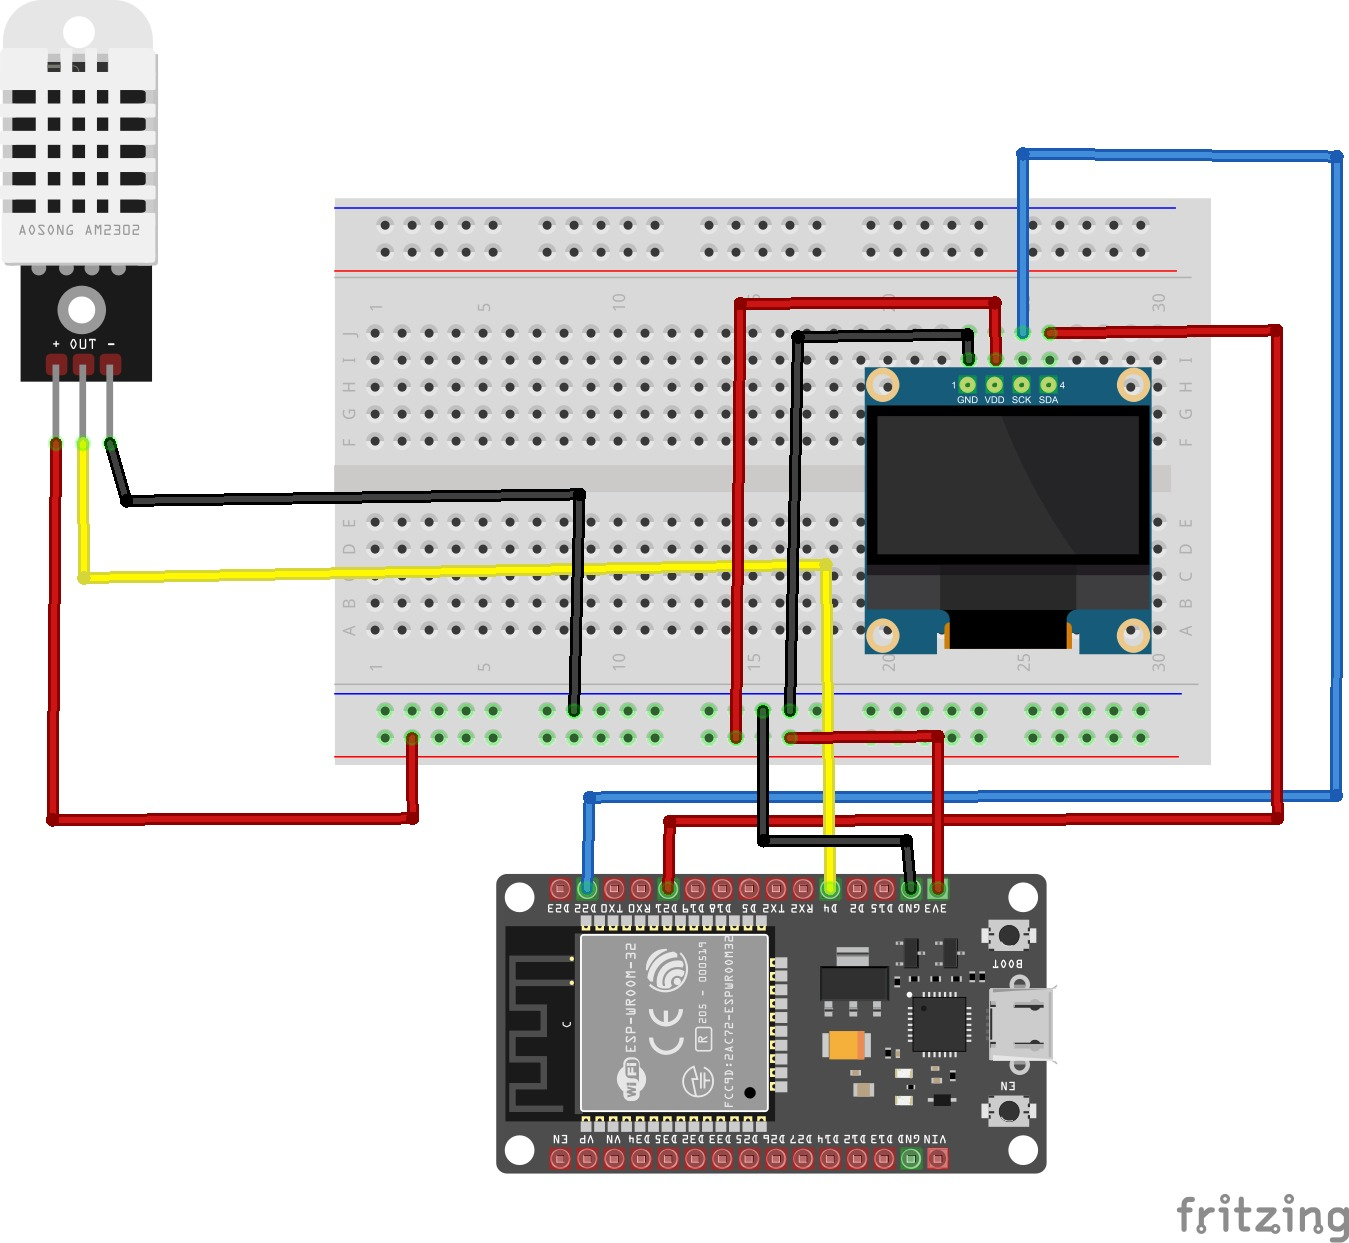
\includegraphics[width=0.85\textwidth]{../Esquemas/Temperatura_esq.jpeg}
\caption{Esquema de conexión del circuito -- Temperatura con Termómetro (Fritzing)}
\label{fig:esquema}
\end{figure}

\subsection{Diagrama de Conexiones}

\begin{center}
\begin{tabular}{lll}
\toprule
\textbf{Componente} & \textbf{Pin} & \textbf{ESP32 GPIO} \\
\midrule
DHT22 & + (VCC) & 3.3V \\
DHT22 & OUT (datos) & GPIO4 \\
DHT22 & -- (GND) & GND \\
OLED SSD1306 & GND & GND \\
OLED SSD1306 & VDD & 3.3V \\
OLED SSD1306 & SCK (SCL) & GPIO22 \\
OLED SSD1306 & SDA & GPIO21 \\
\bottomrule
\end{tabular}
\end{center}

% ══════════════════════════════════════════════════════════════
\section{Código Fuente}
% ══════════════════════════════════════════════════════════════

A continuación se presenta el código completo del proyecto. Se ha organizado en secciones funcionales claramente delimitadas.

\subsection{Código Completo}
\lstinputlisting[language=C++, title=ESP32\_DHT22\_OLED\_ConTermometro.ino]{../Arduino/ESP32_DHT22_OLED_ConTermometro/ESP32_DHT22_OLED_ConTermometro.ino}

% ══════════════════════════════════════════════════════════════
\subsection{Análisis del Código}
% ══════════════════════════════════════════════════════════════

\subsubsection*{Librerías Incluidas}
El programa utiliza cuatro librerías:
\begin{itemize}
    \item \textbf{\texttt{Wire.h}:} Librería nativa para comunicación I2C. Gestiona SDA y SCL.
    \item \textbf{\texttt{Adafruit\_GFX.h}:} Librería gráfica base con primitivas de dibujo (texto, rectángulos, círculos, líneas, rellenos).
    \item \textbf{\texttt{Adafruit\_SSD1306.h}:} Driver específico para pantallas OLED con controlador SSD1306.
    \item \textbf{\texttt{DHT.h}:} Librería para sensores de la familia DHT. El tercer parámetro del constructor (\texttt{22}) es un ajuste de temporización necesario para procesadores rápidos como el ESP32 a 240\,MHz.
\end{itemize}

\subsubsection*{Constantes de Configuración}
\begin{itemize}
    \item \textbf{\texttt{ANCHO = 128}, \texttt{ALTO = 64}:} Resolución de la pantalla OLED en píxeles.
    \item \textbf{\texttt{DIR\_OLED = 0x3C}:} Dirección I2C de la pantalla (alternativa: \texttt{0x3D}).
    \item \textbf{\texttt{PIN\_DHT = 4}:} GPIO4 del ESP32 para la comunicación con el DHT22.
    \item \textbf{\texttt{T\_MIN = 0.0}, \texttt{T\_MAX = 40.0}:} Rango de escala del termómetro gráfico en $^\circ$C.
    \item \textbf{\texttt{INTERVALO\_MS = 2000}:} Pausa de 2 segundos entre lecturas (mínimo del DHT22).
    \item \textbf{\texttt{ultimaT}, \texttt{ultimaH}:} Variables de memoria que almacenan la última lectura válida, inicializadas en \texttt{NAN}.
\end{itemize}

\subsubsection*{Función \texttt{dibujarTermometro(tempC)}}
Esta es la función más relevante del proyecto y la que lo diferencia de la versión básica. Dibuja un termómetro clásico en la esquina izquierda de la pantalla OLED:

\begin{enumerate}
    \item \textbf{Recorte de rango:} Limita \texttt{tempC} al intervalo $[\texttt{T\_MIN}, \texttt{T\_MAX}]$.
    \item \textbf{Geometría:} Define las dimensiones del tubo (\texttt{x\_tubo=4}, \texttt{y\_tubo=4}, \texttt{ancho=10}, \texttt{alto\_tubo=42}) y del bulbo (\texttt{r\_bulbo=7}). Calcula el centro del bulbo como:
    \begin{equation*}
        cx = x_{\text{tubo}} + \frac{\text{ancho}}{2}, \qquad cy = y_{\text{tubo}} + \text{alto\_tubo} + r_{\text{bulbo}} - 1
    \end{equation*}
    \item \textbf{Contorno:} Dibuja el tubo con \texttt{drawRect()} y el bulbo con \texttt{drawCircle()}.
    \item \textbf{Marcas de escala:} Tres líneas horizontales (máximo, medio, mínimo) con \texttt{drawFastHLine()}.
    \item \textbf{Cálculo del nivel:} La proporción del relleno se calcula como:
    \begin{equation*}
        \text{prop} = \frac{T - T_{\min}}{T_{\max} - T_{\min}}, \qquad \text{nivel} = \lfloor \text{prop} \times \text{alto\_tubo} \rfloor
    \end{equation*}
    \item \textbf{Relleno:} El bulbo se rellena siempre con \texttt{fillCircle()}, y la columna de ``mercurio'' con \texttt{fillRect()} desde el nivel calculado hasta la base del tubo.
\end{enumerate}

\subsubsection*{Función \texttt{mostrarDatos(t, h)}}
Orquesta el layout completo de la pantalla:
\begin{itemize}
    \item Limpia la pantalla con \texttt{clearDisplay()}.
    \item Llama a \texttt{dibujarTermometro(t)} para el gráfico izquierdo (x = 4--22).
    \item Muestra las etiquetas ``Temperatura:'' y ``Humedad:'' en tamaño 1 (8 px).
    \item Muestra los valores numéricos en tamaño 2 (16 px) con un decimal.
    \item Usa el carácter ASCII 248 para el símbolo de grado ($^\circ$) en la codificación CP437.
    \item Envía el buffer a la pantalla con \texttt{display()}.
\end{itemize}

\subsubsection*{Función \texttt{setup()}}
\begin{enumerate}
    \item Inicia comunicación serial a 115200 baudios.
    \item Configura I2C con \texttt{Wire.begin(21, 22)}.
    \item Inicializa la OLED; si falla, detiene la ejecución con un bucle infinito.
    \item Inicializa el sensor DHT22.
    \item Muestra pantalla de bienvenida durante 2 segundos.
\end{enumerate}

\subsubsection*{Función \texttt{loop()}}
\begin{enumerate}
    \item Lee temperatura y humedad del DHT22.
    \item Si la lectura es válida, actualiza \texttt{ultimaT} y \texttt{ultimaH} y envía datos por serial.
    \item Si la lectura falla, imprime advertencia pero \textbf{no borra los últimos valores válidos}.
    \item Redibuja la pantalla OLED si existe al menos una lectura válida previa.
    \item Espera 2 segundos antes de la siguiente iteración.
\end{enumerate}

\textbf{Nota importante:} A diferencia de la versión sin termómetro, este código implementa un patrón de \textit{último valor válido}: las variables \texttt{ultimaT} y \texttt{ultimaH} conservan la última lectura exitosa, de modo que una falla puntual del sensor no vacía la pantalla.

% ══════════════════════════════════════════════════════════════
\section{Principio de Funcionamiento}
% ══════════════════════════════════════════════════════════════

\subsection{Comunicación con el Sensor DHT22}
El DHT22 utiliza un protocolo propietario de un solo hilo (\textit{single-wire}):
\begin{enumerate}
    \item El ESP32 envía una señal de inicio: \texttt{LOW} durante al menos 1\,ms, luego libera la línea.
    \item El DHT22 responde con confirmación (\texttt{LOW} 80\,$\mu$s + \texttt{HIGH} 80\,$\mu$s).
    \item Transmite 40 bits: cada bit comienza con \texttt{LOW} (50\,$\mu$s) seguido de \texttt{HIGH}. La duración del pulso alto determina el valor: 26--28\,$\mu$s = ``0'', 70\,$\mu$s = ``1''.
    \item Distribución: 16 bits humedad + 16 bits temperatura + 8 bits checksum.
\end{enumerate}

\subsection{Comunicación I2C con la Pantalla OLED}
El protocolo I2C utiliza dos líneas:
\begin{itemize}
    \item \textbf{SDA (GPIO21):} Línea bidireccional de datos.
    \item \textbf{SCL (GPIO22):} Línea de reloj generada por el maestro (ESP32).
\end{itemize}
La pantalla responde en la dirección \texttt{0x3C}. Los comandos y datos de píxeles se envían mediante tramas I2C estándar.

\subsection{Renderizado Gráfico del Termómetro}
El termómetro se renderiza mediante primitivas gráficas de la librería \texttt{Adafruit\_GFX}. El proceso de mapeo de temperatura a píxeles sigue una interpolación lineal:

\begin{equation}
y_{\text{nivel}} = y_{\text{tubo}} + \text{alto\_tubo} - \left\lfloor \frac{T - T_{\min}}{T_{\max} - T_{\min}} \times \text{alto\_tubo} \right\rfloor
\label{eq:nivel}
\end{equation}

Esto significa que a mayor temperatura, el nivel $y_{\text{nivel}}$ es menor (más arriba en la pantalla), creando la ilusión visual de que el ``mercurio'' sube. El bulbo inferior siempre permanece lleno, simulando el depósito de mercurio de un termómetro real.

El layout de la pantalla se distribuye así:
\begin{verbatim}
    +--------------------------------+
    |   XXX  Temperatura:            |
    |  X   X    25.6°C               |
    |  X   X                         |
    |  X###X  Humedad:               |
    |  X###X    62.3 %               |
    |  X###X                         |
    |  X###X                         |
    |   ###                          |
    +--------------------------------+
     Termómetro         Valores
     (0-40°C)         (tamaño x2)
\end{verbatim}

% ══════════════════════════════════════════════════════════════
\section{Fotografías del Montaje}
% ══════════════════════════════════════════════════════════════

Las siguientes imágenes muestran el proyecto montado y en funcionamiento. Se puede observar el ESP32 montado sobre su placa de expansión con borneras, el sensor DHT22 conectado en la protoboard, y la pantalla OLED mostrando el termómetro gráfico junto con los valores de temperatura y humedad.

\begin{figure}[H]
\centering
\begin{subfigure}[b]{0.48\textwidth}
    \centering
    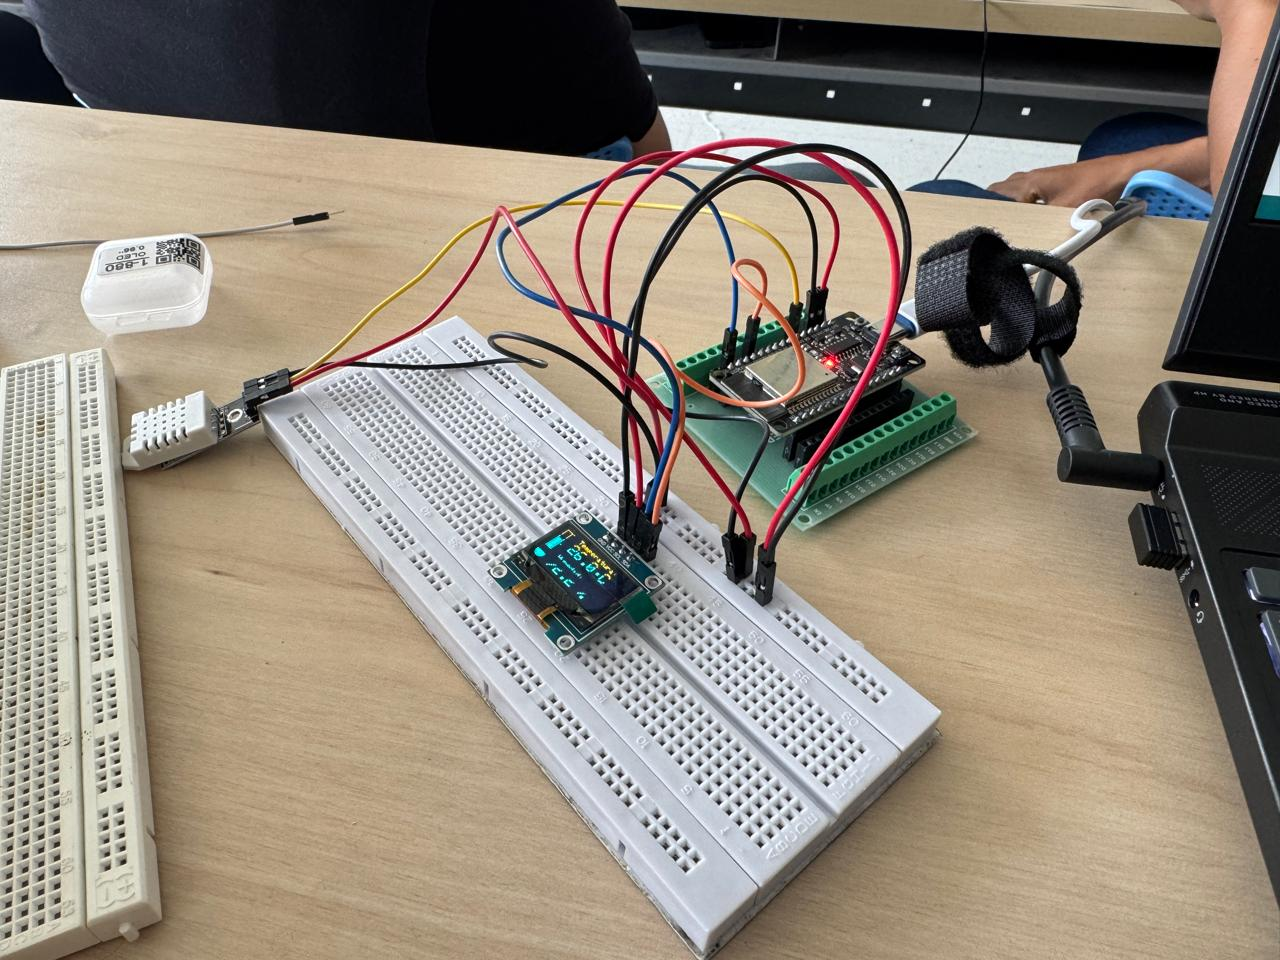
\includegraphics[width=\textwidth]{../Imagenes/Temperatrua_Con_termometro_imgs/Temperatrua_con_termometro_img1.jpeg}
    \caption{Vista general del montaje con ESP32, DHT22 y pantalla OLED}
    \label{fig:montaje1}
\end{subfigure}
\hfill
\begin{subfigure}[b]{0.48\textwidth}
    \centering
    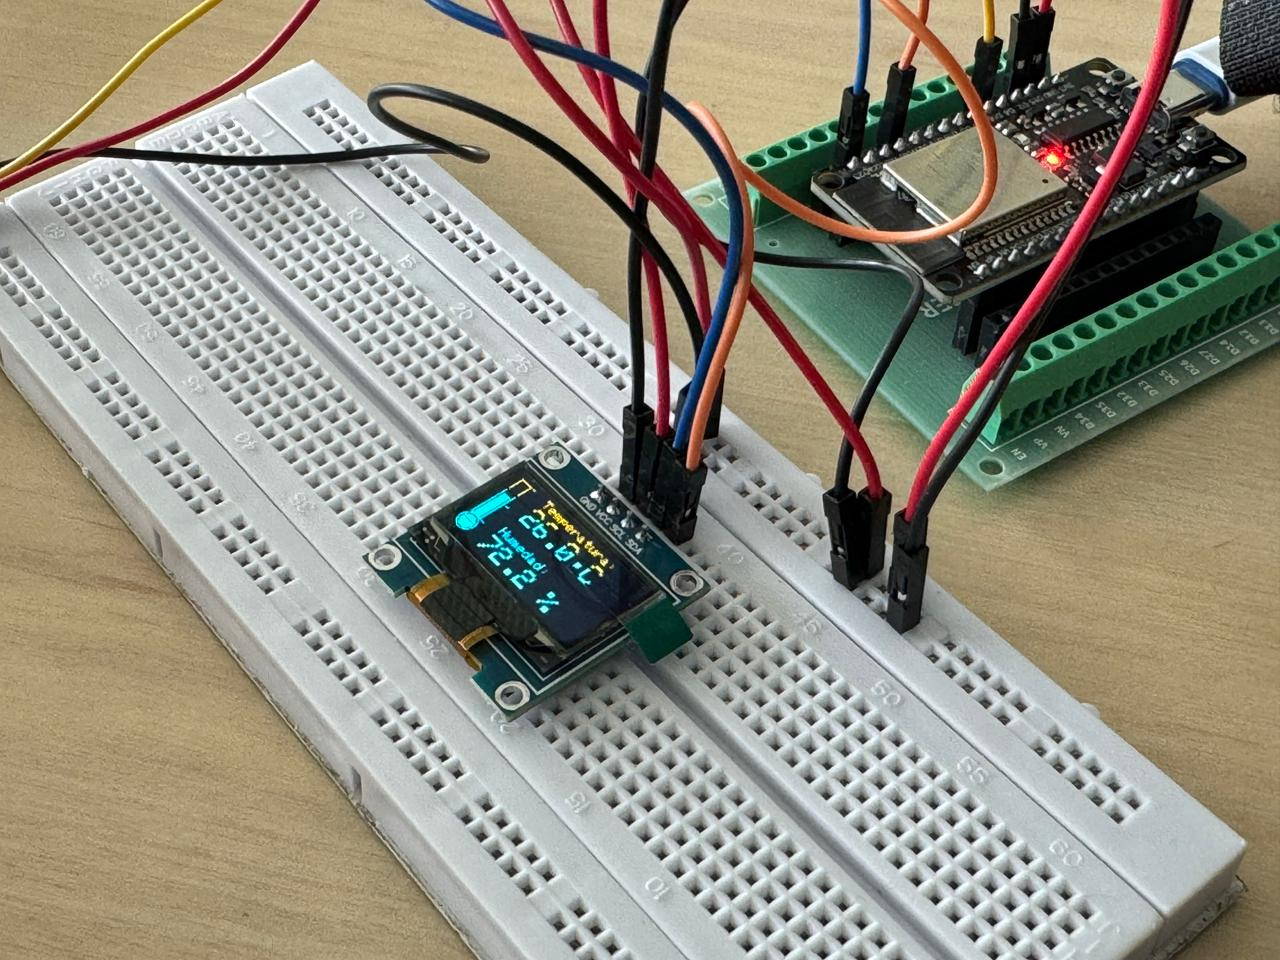
\includegraphics[width=\textwidth]{../Imagenes/Temperatrua_Con_termometro_imgs/Temperatrua_Con_termometro_img2.jpeg}
    \caption{Detalle de la pantalla OLED mostrando el termómetro gráfico}
    \label{fig:montaje2}
\end{subfigure}
\caption{Montaje físico del proyecto Temperatura con Termómetro}
\label{fig:montaje}
\end{figure}

En la Figura~\ref{fig:montaje2} se aprecia claramente el termómetro gráfico a la izquierda de la pantalla OLED, con el nivel de ``mercurio'' correspondiente a la temperatura ambiente, y los valores numéricos de temperatura y humedad a la derecha.

% ══════════════════════════════════════════════════════════════
\section{Proceso de Creación}
% ══════════════════════════════════════════════════════════════

El desarrollo de este proyecto siguió los siguientes pasos:

\begin{enumerate}
    \item \textbf{Selección de componentes:} Se reutilizó el mismo hardware del proyecto base (ESP32 + DHT22 + OLED SSD1306), demostrando que las mejoras son puramente de software.
    
    \item \textbf{Diseño del circuito:} Se mantiene el mismo esquema de conexiones diseñado en Fritzing (Figura~\ref{fig:esquema}).
    
    \item \textbf{Diseño del layout gráfico:} Se planificó la distribución de la pantalla de 128$\times$64 píxeles, asignando los primeros 22 píxeles horizontales al termómetro y el resto a los valores numéricos.
    
    \item \textbf{Implementación del termómetro gráfico:} Se desarrolló la función \texttt{dibujarTermometro()} utilizando las primitivas de \texttt{Adafruit\_GFX}:
    \begin{itemize}
        \item \texttt{drawRect()}: contorno del tubo.
        \item \texttt{drawCircle()}: contorno del bulbo.
        \item \texttt{drawFastHLine()}: marcas de escala.
        \item \texttt{fillCircle()}: relleno del bulbo (siempre lleno).
        \item \texttt{fillRect()}: columna de mercurio (proporcional a T).
    \end{itemize}
    
    \item \textbf{Mejora del manejo de errores:} Se implementó el patrón de ``último valor válido'' con las variables \texttt{ultimaT} y \texttt{ultimaH}, evitando que la pantalla se vacíe ante lecturas fallidas.
    
    \item \textbf{Calibración del rango visual:} Se definió T\_MIN = $0\,^\circ$C y T\_MAX = $40\,^\circ$C como rango del termómetro, adecuado para el clima de Cartago (Valle del Cauca).
    
    \item \textbf{Configuración del Arduino IDE:}
    \begin{itemize}
        \item Placa: \textit{ESP32 Dev Module}.
        \item Velocidad de subida: 115200 baudios.
        \item Puerto: COM correspondiente al ESP32 conectado.
    \end{itemize}
    
    \item \textbf{Pruebas y validación:} Se verificó el correcto funcionamiento del termómetro gráfico en diferentes condiciones de temperatura, confirmando la proporcionalidad visual del nivel de mercurio.
\end{enumerate}

% ══════════════════════════════════════════════════════════════
\section{Diferencias con el Proyecto Base}
% ══════════════════════════════════════════════════════════════

\begin{table}[H]
\centering
\begin{tabular}{lcc}
\toprule
\textbf{Característica} & \textbf{Sin Termómetro} & \textbf{Con Termómetro} \\
\midrule
Representación visual & Solo texto & Termómetro gráfico + texto \\
Dirección I2C & 0x7A & 0x3C \\
Manejo de errores & Muestra error & Último valor válido \\
Layout pantalla & Texto centrado & Gráfico izq. + texto der. \\
Funciones gráficas & Ninguna & drawRect, fillCircle, etc. \\
Rango de escala & No aplica & 0--40$\,^\circ$C configurable \\
Pantalla de bienvenida & Básica & Con nombre del proyecto \\
\bottomrule
\end{tabular}
\caption{Comparación entre las dos versiones del proyecto de temperatura}
\end{table}

% ══════════════════════════════════════════════════════════════
\section{Conclusiones}
% ══════════════════════════════════════════════════════════════

\begin{itemize}
    \item El proyecto demuestra cómo crear interfaces gráficas informativas en pantallas OLED de resolución limitada, combinando representaciones visuales (termómetro) con datos numéricos.
    \item La función \texttt{dibujarTermometro()} ilustra el mapeo lineal de magnitudes físicas a coordenadas de píxeles, un concepto fundamental en visualización de datos y sistemas embebidos.
    \item El patrón de ``último valor válido'' mejora significativamente la robustez del sistema frente a lecturas fallidas del sensor.
    \item Las primitivas gráficas de \texttt{Adafruit\_GFX} permiten crear interfaces ricas sin necesidad de imágenes bitmap, optimizando el uso de memoria del microcontrolador.
    \item El rango configurable del termómetro (T\_MIN/T\_MAX) permite adaptar la visualización a diferentes contextos climáticos y aplicaciones.
    \item Este proyecto demuestra que mejoras significativas en la experiencia de usuario pueden lograrse exclusivamente mediante software, sin modificar el hardware.
\end{itemize}

\end{document}
